\documentclass{article}
\usepackage{parskip}
\usepackage{pdfpages}
\usepackage[margin=.6in]{geometry}
\begin{document}

\includepdf[pages=1-3]{slides}
We talked about the ways that life might have occurred on earth. Its very probably that it happened without outside force, which means that it could happen on other planets.


\includepdf[pages=3-6]{slides}
Just remember the shit from astro 101.


\includepdf[pages=7-8]{slides}
The kind of start determines where the habitable zone is, habitable zone is just where liquid water can exist.


\includepdf[pages=9-14]{slides}
Exoplanets are very hard to detect because they only emit reflected light from their sun, but the star is so powerful it hides the planet. We dont really see them, instead we have indirect proof.

The planets subtly alter the stars location due to the effect of gravity and we can see this wobble. The sun should give off perfect light but there are little spots in the atomic spectrum there are tiny particles in the star's atmosphere and we can use these spots to see if the star is red shifted or blue shifted and from this we can see if the star is moving closer or farther from us. This is how we measure the wobble and know how the star is moving. This gives us the mass of the planet. We can use the period of the wobble to know how far the planet from the sun. This will tell us if it is in the habitable zone.


\includepdf[pages=15]{slides}
We can also learn alot about planets that are planar to us.


\includepdf[pages=16]{slides}

\includepdf[pages=17]{slides}
We frequently compare the planet's density to water. We know this because we can get its size and mass. Its crazy what we know.


\includepdf[pages=18]{slides}
The kepler mission was awesome. It brought back a ton of data. For instance this is the orbital time for known planets (we need three sightings for this).11


\includepdf[pages=19]{slides}
Its much easier to see planets that are closer to their star so we have more data on them.

The green band on the second picture shows where liquid water might exist.


\includepdf[pages=20]{slides}

\includepdf[pages=21]{slides}
We recently discovered some very promising planets.

\includepdf[pages=22-27]{slides}

Potential question for assignment = \emph{could life evolve on a water world?}


\includepdf[pages=28-32]{slides}
For life to exist all the laws that we have have to be the same, but these are universal laws so its reasonable.


\includepdf[pages=33-42]{slides}
Life on early basically happened immediately after the late heavy bombardment caused the right conditions. This implies that the transition between chemestry and biology is easier than we think.


\includepdf[pages=43]{slides}
When we looke at the rates of oxygen throughout the history of earth we can see that there have been 5 massive extinctions. Right after these dips we see spikes implying that life comes right back up after the extinction.


\includepdf[pages=44-46]{slides}


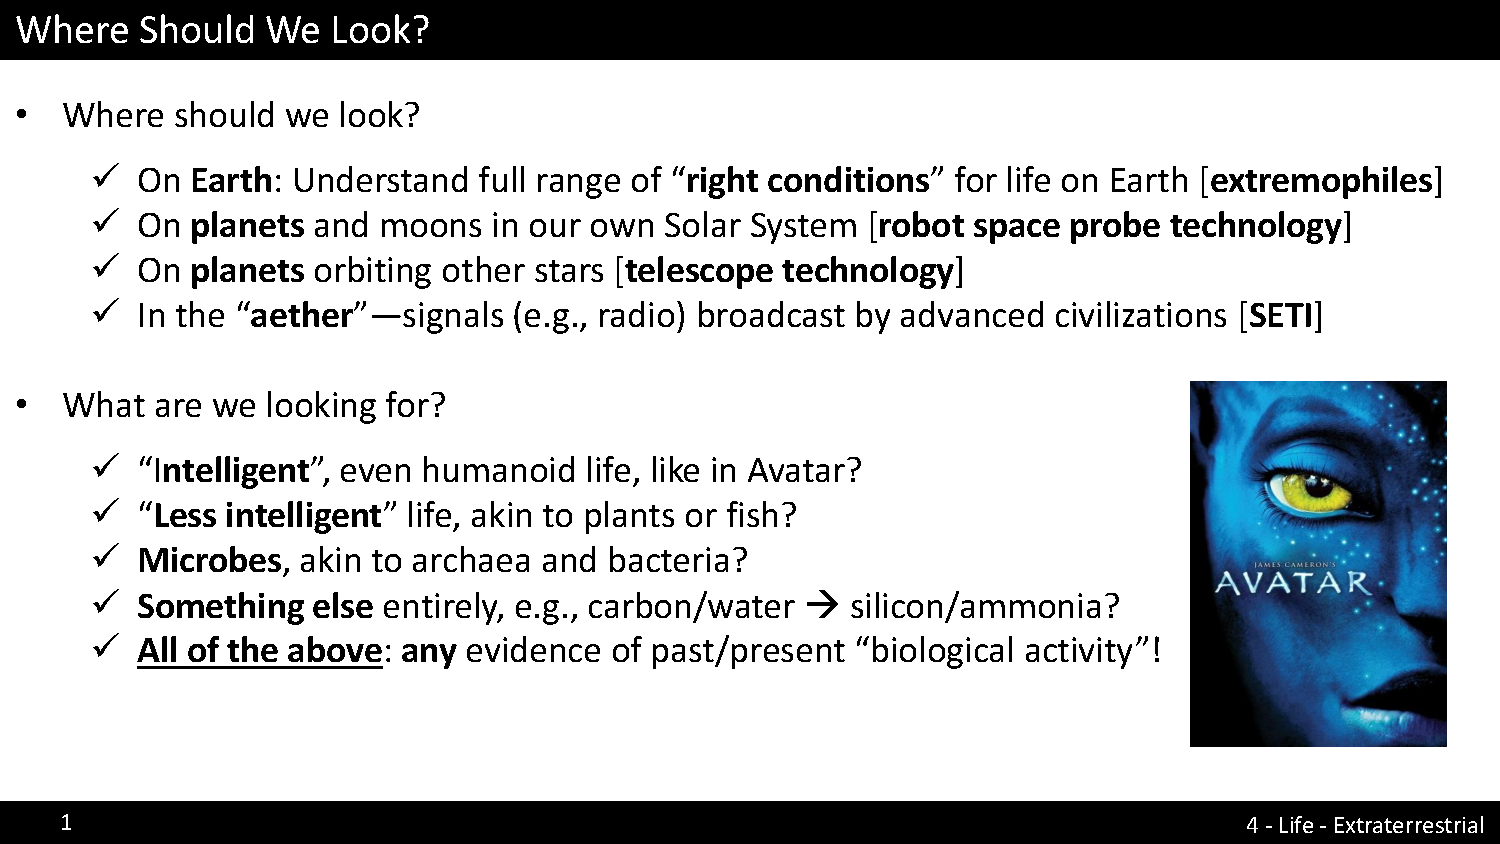
\includepdf[pages=1-2]{slides2}
Its possible that we could have life arrive under different circumstances, using different elements. Life only uses 25/92 of the naturally ocurring elements,

\includepdf[pages=3-4]{slides2}
We need liquid because stuff as to move around to break things down and reform them. They are required for transporting things used in the processes of life. Water in particular is very important because it has many unique properties (is polar for dissolving, made of common elements, is less dense when frozen).

\includepdf[pages=5]{slides2}
If you have life in a cold liquid its metabalism is slower and vice versa.

\includepdf[pages=6]{slides2}
Titan has rocks made out of water and an nitrogen rich atmosphere.

\includepdf[pages=7]{slides2}
One of most important things needed for life is actually just the weird fact that neutrons weigh more than protons. Without this we couldnt really get chemisty rolling. From there we get the molecules neded to build organisms.

\includepdf[pages=8]{slides2}
We need chemestry to build organisms, a source of free energy to fuel metabolism, and finally a liquid medium to move stuff around in. The first two conditions are not all that uncommon, one is a universal rule the other comes from stars, so the main limiting feature is the presence of water. Weirdly enough we also need tidal forces.

\includepdf[pages=9]{slides2}
Without an atmosphere on the moon there is no way to distribute the temperature which causes immense temperature fluctuations during the day. Water also helps even out the heat. The moon does have water, but its frozen on the poles.

\includepdf[pages=10]{slides2}
Believe it or not, life is more likely on venus. It has an atmosphere which actually heats everything up due to how dense the air is. The soviets sent a probe which landed on it and then immidiately melted. There are continents and TONS of volcanoes. There is other evidence of techtonic activity. We known that there was a time of immense technonic shifting which means that any proof of life is surely lost.

\includepdf[pages=11]{slides2}
Venus has a run away greenhouse effect. The two planets are very similiar and had nearly identical starts. The initial atmosphere was formed the same way (volcanoes spewing water vapor). Earth is slightly cooler which allows the water to form clouds and make rain which then makes oceans and the whole water cycle shebang. The water in the atmosphere helps to dissolve C02 out of the atmosphere and rain it down into the ocean. This C02 in the ocean gets seemed into rocks, these rocks then get subducted under the crust and are then spewed into the atmosphere in a C02 cycle.

Venus is much warmer than earth which prevents it from the equilibrium needed for a sustainable cycle. More water evaporated than rained which resulted in the oceans drying up so there was no way to scrub C02 from the atmosphere which causes the run away greenhouse effect. The excessive radiation dissassociates the water into hydrogen and oxygen, the hydrogen escapes and the oxygen reacts with carbon in the rocks to make C02.

\includepdf[pages=12]{slides2}
\includepdf[pages=13]{slides2}
It looks like mars is a bit warmer than earth and started with a slightly thicker atmosphere. It was also fairly wet as well. The planet is slightly smaller than earth which lowered the pressure of the atmosphere which caused water to boil away.

\includepdf[pages=14]{slides2}
Mars is half the diameter of earth, so a quarter of the surface area and one eighth the volume. This means the ratio of surface are to volume is twice that of earth. Remember that planets are full of molten rock. Since its volume is much less it has less internal area but has way more surface area (ratio wise) to give off all the energy it had. This resulted in the end of volcanic energy and the loss of its magnetic field (the center is no longer liquid and thus no longer spinning). This contributed to the loss of the atmosphere because the magnetic field no long deflected the charged particles from the sun. Due to the loss of the atmosphere there is also no ozone layer so the surface gets fucked by UV rays. So unlike venus mars lost all of its greenhouse effects which caused it to be very cold and dry.

\includepdf[pages=15-20]{slides2}
Theres tons of ice at the poles of mars, most of it is water ice but some is carbon dioxide ice. Mars is tilted like earth so it has seasons. So during the summer the carbon dioxide turns into gas, a very large portion actually. So the atmosphere flows from the south pole and causes some real cool dust storms. Theres a fair amount of water that we can see on the surface (enough to cover the planet in 35m of water) and even more underground.

\includepdf[pages=21-26]{slides2}
The immense pressure on these gas giants causes hydrogen to crystallize in a weird latice structure which forms the core.

\includepdf[pages=27]{slides2}
It rains helium droplets which is boss.

\includepdf[pages=28]{slides2}
Life is unlikely. There is no solid ground so if you fell into the planet until you matched the desity of the hydrogen around you. To get hydrogen as dense as water it takes tons of pressure which would make it about as hot as the surface of the sun. Its possible that the right conditions exist, but not statically.

\includepdf[pages=29]{slides2}
Europa gets tidal forces from jupiter which keeps bending the rock around it but this friction warms up the moon. The theory is that this could lead to a liquid ocean.

\includepdf[pages=30]{slides2}
The surface looks solid with a bunch of cracks all over the place but under it there is probably liquid oceans. We currently dont know what kind of ocean it might be. These flowing oceans could create a magnetic field. We know that the water is salty based on the strength of the magenetic field. It is possible that this is enough to support simple life.

\includepdf[pages=31]{slides2}
Titan has a very thick organic rich atmosphere. There is a rocky core and water stuff on top if it. Its under super high pressure so its solid. Due to the extreme cold this surface would be hard as granite.

\includepdf[pages=32-33]{slides2}
Has the thickest atmosphere of the moons in our solar system. Its also very chemically active. In 2013 we landed on the surface. By using radar we can identify where there are liquids (they are perfectly flat and thus reflect a certain way) so we think there might be methane oceans.

\includepdf[pages=34-36]{slides2}
We can learn alot about a planet just from observing the light being emited from it.

\includepdf[pages=37]{slides2}
Life dramatically changes the atmosphere of a planet so we can mimic what earth's atmosphere would be at different times to see how life effected it,

\includepdf[pages=38-42]{slides2}


\includepdf[pages=1-2]{slides}
We are listening really hard to hear when aliens contact us since we are a long way off from us contacting them.


\includepdf[pages=3-7]{slides}










\end{document}
